\chapter{Analyses}
In this chapter, an analysis of the data collected via the methods described in
the previous chapter (Chapter~\ref{ch:Methods}) is given. Firstly, a brief
initial overview is provided, where descriptive statistics of the equilibria
obtained and the overall characteristics of the strategies used is discussed.
Following this, a critical analysis of the p-thresholds obtained is carried out.
Here, the environmental effects, on the outcome of the game, discussed include:
number and characteristics of opponents; noise; and degeneracy. Then a
large-scale multivariate analysis is executed before considering the reliability
of the collected data. Note, as of writing, the database currently has 
\input{../../../src/database-code/data/se/20_01_2020/entries-in-database.txt}
entries (rows) and a total number of \input{../../../src/database-code/data/se/20_01_2020/number-of-tournaments} tournament sets.

\section{Initial Analysis}
In this section, all the data (including those games which could be degenerate)
are considered. Taking a brief look at the graphs produced for each game, it can
be seen that the main `shapes' obtained are as seen in
Figure~\ref{fig:example_graphs}.

\begin{figure}
    \centering
    \begin{subfigure}[0.3\textwidth]
        \centering
        \includegraphics[width=\textwidth]{folk_thm/single_game/2/0/0.0/main.pdf}
        \caption{An example of a graph with a clear p-threshold point of approximately 0.28. In this game there is no degeneracy and the opponent strategy playing in the tournament was Inverse, without noise.}
    \end{subfigure}
    \begin{subfigure}[0.3\textwidth]
        \centering
        \includegraphics[width=\textwidth]{folk_thm/single_game/6/110/0.0/main.pdf}
        \caption{An example of a graph where the p-threshold is not as clear, perhaps due to a small amount of noise and hence not enough repetitions. In this case the threshold seems to lie in the range [0.1, 0.3]. There is no degeneracy in this game and opponent strategies in the tournament were: Feld: 1.0, 0.5, 200; Cooperator;  EvolvedLookerUp2_2_2; Tullock: 11; and ZD-GEN-2: 0.125, 0.5, 3. Again, this tournament was run with no added noise.}
    \end{subfigure}
\end{figure}

\section{Analysis of the p-Threshold}

\subsection{Effects of the Number of Players}

\subsection{Effects of Stochastic Players}

\subsection{Effects of Noise}

\subsection{Effects of Degeneracy}

\section{Multivariate Data Analysis}

\section{Reliability of Data}

\subsection{Comparison of Databases}

\subsection{Accuracy of Thresholds}